\documentclass[conf]{new-aiaa}
%\documentclass[journal]{new-aiaa} for journal papers
\usepackage[utf8]{inputenc}

\usepackage{graphicx}
\usepackage{amsmath}
\usepackage{sidecap}
\usepackage[version=4]{mhchem}
\usepackage{siunitx}
\usepackage{longtable,tabularx}
\setlength\LTleft{0pt} 

\title{A Convex Optimal and LQG Control Approach for Quadcopters}

\author{ Pádraig Lysandrou
\footnote{Undergraduate Student, Electrical and Computer Engineering, AIAA Student Member \\ A final project for MAE6780: Multivariate Control Theory}}

\affil{Cornell University, Ithaca, New York, 14853}


\begin{document}

\maketitle

\begin{abstract}
In this paper, I present the theory behind and implementation of a neighbouring optimal Linear Quadratic Gaussian quadcopter controller with convex optimal guidance trajectories. My LQG solution uses an Extended Kalman Filter for optimal nonlinear estimation. I employ the convex optimization machinery as the guidance algorithm to generate paths of minimum energy consumption. This work is motivated by applications which require efficient use of energy. This includes autonomous delivery, mapping missions, search and rescue, swarm path planning, and many more. The ultimate goal of this project was to design and simulate a functioning LQG controller that follows convex optimal trajectories with high accuracy and amenable to implementation on my own physical autonomous hardware platforms. I would like my solution to be extensible to more complicated tasks in the future.

 The convex optimal guidance works well taking approx (time completion per meter), and the LQG controller converges and accurately trackes trajectories (some metric).
\end{abstract}

\section*{Nomenclature}

{\renewcommand\arraystretch{1.0}
\noindent\begin{longtable*}{@{}l @{\quad=\quad} l@{}}
$A$  & amplitude of oscillation \\
$a$ &    cylinder diameter \\
$C_p$& pressure coefficient \\
$Cx$ & force coefficient in the \textit{x} direction \\
$Cy$ & force coefficient in the \textit{y} direction \\
c   & chord \\
d$t$ & time step \\
$Fx$ & $X$ component of the resultant pressure force acting on the vehicle \\
$Fy$ & $Y$ component of the resultant pressure force acting on the vehicle \\
$f, g$   & generic functions \\
$h$  & height \\
$i$  & time index during navigation \\
$j$  & waypoint index \\
$K$  & trailing-edge (TE) nondimensional angular deflection rate
\end{longtable*}}


\clearpage
\begin{doublespace}

\section{Introduction and Theory}
The goal of this project was to design and simulate a functioning LQG controller that follows convex optimal trajectories with high accuracy. Additionally, I wanted the algorithm to be amenable to implementation on my own quadrotor platforms. To reach this goal, I chose a control solution that could be implemented online and would be simple to implement on an embedded system such as an ARM Cortex microcontroller with interrupt service routine timers. Due to Wonham's separation principle, which I will discuss later, the stochastic version of the LQR controller can be split up into an optimal regulator (LQR) and an optimal estimator in the form of a Kalman Filter. If both are stable, then the whole control solution is stable. In my implementation, I write my own finite time horizon LQR using the Riccati matrix equation. Additionally, I have written my own Extended Kalman Filter (EKF) utilizing nonlinear state propagation via our dynamical equations. For the theory section, I will be covering the quadrotor dynamics, derivation of the LQG controller, introducing convex optimization, and the derivation of my own convex problem proposition.

Before we develop the control system, we must first create a dynamic model for the system. The frame of the vehicle is a cross-shape with four motor/propeller combinations, one on each end. In figure 1, we see that if we increase the thrust similarly on F1/F2 or F3/F4 the vehicle rolls right or left respectively, as a torque is applied to the system. Additionally we see that if we increase the thrust produced by F4/F1 or F3/F2 the quadrotor pitches forward or backward respectively. The rotor speeds can be increased or decreased to produce a yaw on the vehicle with the conservation of angular momentum. 


\begin{figure}[!h]
	\centering
	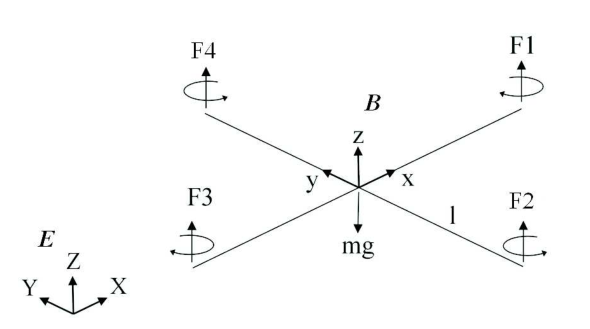
\includegraphics[scale= 0.45]{quad.png}
	\caption{Quadrotor Layout with body fixed frame B and inertial frame E}
	\label{fig:f1}
\end{figure}
	
\begin{SCfigure}[1][!ht] 
	\begin{minipage}{0.25\textwidth}
		\begin{equation*}\label{fig:eq1}
			\begin{cases}
				& \dot{\xi} = \nu \\
				& m\dot{v} = RF_b \\
				& \dot{R} = R\hat{\omega} \\
				& J\dot{\omega} = -\omega \times J\omega + \tau_a
			\end{cases}
		\end{equation*}
	\end{minipage}
  \begin{minipage}{.35\textwidth}
    \begin{align*}
        &\ddot{x}=(\cos\phi\sin\theta\cos\psi + \sin\phi\sin\psi)\frac{U_1}{m} \\
		&\ddot{y}=(\cos\phi\sin\theta\sin\psi - \sin\phi\cos\psi)\frac{U_1}{m} \\
		&\ddot{z}=(\cos\phi\cos\theta)\frac{U_1}{m} -g \\
		&\ddot{\phi} = \dot{\theta}\dot{\psi}\Big(\frac{I_y - I_z}{I_x}\Big) - \frac{J_r}{I_x}\dot{\theta}\Omega + \frac{l}{I_x}U_2\\
		&\ddot{\theta} = \dot{\phi}\dot{\psi}\Big(\frac{I_z - I_x}{I_y}\Big) - \frac{J_r}{I_y}\dot{\phi}\Omega + \frac{l}{I_y}U_3 \\
		&\ddot{\psi} = \dot{\phi}\dot{\theta}\Big(\frac{I_z - I_y}{I_z}\Big) + \frac{1}{I_z}U_4
    \end{align*}
  \end{minipage}%
  \begin{minipage}{.3\textwidth}
  	\begin{align*}
  		&U_1 = b(\Omega_1^2 + \Omega_2^2 + \Omega_3^2 +\Omega_4^2)\\
  		&U_2 = b(\Omega_4^2 -\Omega_2^2) \\
  		&U_3 = b(\Omega_3^2 - \Omega_1^2) \\ 
  		&U_4 = d(\Omega_2^2 + \Omega_4^2 - \Omega_1^2 - \Omega_3^2) \\ 
  		&\Omega = \Omega_2 + \Omega_4 - \Omega_1 - \Omega_3
  	\end{align*}
  \end{minipage}
    	\caption{Governing Dynamical Equations}
\end{SCfigure}

$U_1, U_2, U_3, U_4,$ and $\Omega$ represent the inputs of the system: total thrust, roll thrust, pitch thrust, and yaw thrust. The first set of equations in the curly braces (\textbf{equations \ref{fig:eq1}}) show the overall simplified dynamics. Onve the  thrust is distributed in the intertial frame, we can write the dynamics as the second set of equations shown. These are nonlinear, 6 degree of freedom, coupled dynamical equations. The set of equations on the far right describes





5 pages!!
Short introduction
DYNAMICS
FIND AN LQG DERIVATION WITH DYNAMIC PROGRAMMING...
SHOW THE SEPARATION PRINCIPLE
THEN DERIVE THE KALMAN FILTER
THEN DO EXTENDED KALMAN FILTER
SHOW THE BACKGROUND OF CONVEX OPTIMIZATION

\section{Procedure}
5 pages!!
Describe the process  that I took to come to my control solution
describe the simulink blocks and code
with the intention of giving step-by-step instructions to someone

\section{RESULTS}
4 pages
results from the simulations and controllers

Include a description of simulation findings, using diagrams, figures, and numerical data measurements (by means of tables) that provide a convincing argument on the effectiveness and shortcomings of
your chosen multivariable controller, in the context of the original design objectives. 

It may be appropriate to put some of the raw data into Appendices. Plot the results in a meaningful way- “a plot is worth a thousand words,” do NOT underestimate the power of a good plot! Consider using statistical analysis if appropriate when completing a plot. Verify your findings through the theory. Possible causes of error should also be addressed in the concluding paragraph.


\section{Conclusions}
1 paragraph
main contributions, and causes of error, theoretical findings
summary of control performance
what to do in the future

\section{ref}
Be sure to cite any references you used in this lab report using approved IEEE standards. 





\end{doublespace}
\bibliography{sample}
\end{document}
